\documentclass[12pt,a4paper]{article}
\usepackage[utf8]{inputenc}
\usepackage{amsmath}
\usepackage{amsfonts}
\usepackage{amssymb}

%bold Greek letters and other symbols
\usepackage{bm}
\usepackage{graphics}
\usepackage[T1]{fontenc}
\usepackage[english]{babel}
\usepackage{graphicx}
\usepackage[left=2.5cm,right=3.0cm,top=2.5cm,bottom=3cm]{geometry}
\usepackage{color}
%
\usepackage{makeidx}
\usepackage{shortvrb,latexsym}

\setlength{\parindent}{0pt}
%\renewcommand{\floatpagefraction}{.99}
%\renewcommand{\textfraction}{.01}
\def \oo {\bm{\omega}}
\def \curl {\bm{\nabla}\times}
\def \dive {\bm{\nabla}\cdot}
\newcommand{\bu}{\bm{u}}
\newcommand{\bv}{\bm{v}}
\newcommand{\rd}{\mathrm{d}}
\newcommand{\hx}{{\bf\hat{x}}}
\newcommand{\hy}{{\bf\hat{y}}}
\newcommand{\hz}{{\bf\hat{z}}}
\newcommand{\hr}{{\bf\hat{r}}}
\newcommand{\hn}{{\bf\hat{n}}}

\begin{document}

\begin{center}
2020-06-16
\end{center}
STOCKHOLMS UNIVERSITET\\
Meteorologiska Institutionen\\
Jonas Nycander, Dhrubaditra Mitra\\
\vspace{1cm}

\begin{center}
{\bf\large Exam in Fluid mechanics (MO5001)}\\
\end{center}

Write the solution of each problem on a separate paper, and write your identification number on every paper.\\

{\bf Allowed aids:} calculator, sheet with vector analysis relations.\\

{\bf Grading:} A 90-100\%, B 80-89\%, C 65-79\%, D 55-64\%, E 50-54\%, Fx 45-49\%, F 0-44\% \\
\vspace{0.5cm}

\begin{enumerate}

\item \label{prb1} Answer the following short questions. You just need to write the final answer. Each question is worth 3 points. 
  \begin{enumerate}
  \item A vector field, $\bu$, with components $u_x$, $u_y$ and $u_z$,  as a function  of
    space (described by $x$, $y$, and $z$ coordinates )
    is give by the following expression
    \begin{eqnarray}
      u_x &=& \alpha [2x + \sin(y) + 5z^3 ] \nonumber \\
      u_y &=& \alpha[ e^{-x} - y + \cos(z) ] \nonumber \\
      u_z &=& \alpha[ \sin(x) + \cos(y) -z ]
    \end{eqnarray}
   Let $\oo = \curl \bu$. Calculate $\dive \oo$. 
 \item A velocity field $\bu$ in two-dimensions $(x,y)$ is given by the following expression
   \begin{subequations}
     \begin{align}
     u_x &= Sy -x \\
     u_y &= y  \/.
     \end{align}
     \label{eq:uu}
   \end{subequations}
   Calculate the gradient matrix $ G_{\alpha\beta} \equiv \partial_{\beta}u_{\alpha}$, where
   $\partial_{\beta}$ denote spatial derivative, as a function of $x$ and $y$. Is this velocity
   field incompressible ? 
 \item From Eq.~\ref{eq:uu}  calculate vorticity and rate-of-strain as a function of
   space coordinates, $x,y$.
 \item Which of the following are true ? (More than one may be true. )
   Viscosity of a Newtonian fluid is
   \begin{enumerate}
   \item a scalar.
   \item can be described by two scalar quantities.
     \item is a fourth rank tensor. 
    \end{enumerate}
 \item Which of the pictures in figure~\ref{fig:blayer} (left, middle, or right ) shows separation
   of laminar boundary layer ?
  \end{enumerate}
  \begin{figure}
    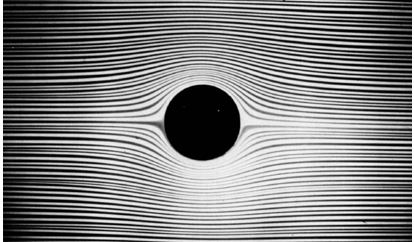
\includegraphics[width=0.3\linewidth]{b1.JPG}
    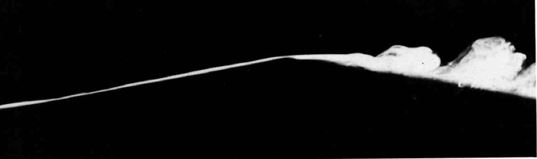
\includegraphics[width=0.3\linewidth]{b2.JPG}
    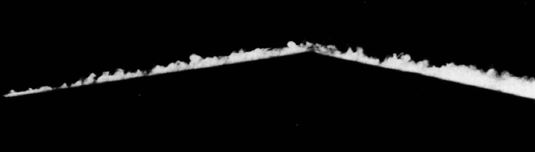
\includegraphics[width=0.3\linewidth]{b3.JPG}
    \caption{\label{fig:blayer}  }
  \end{figure}
\item ({\bf 5 pt}) A cylindrical vessel of height $h$ and base area $S$ is filled with water. An orifice of
  area $s \ll S$ is opened in the bottom of the vessel. Neglecting the viscosity of water determine
  how soon all the water will pour out of the vessel. You make need to make additional
  assumptions other than ignoring the viscosity. Please state them clearly.
  If you do an experiment to verify your calculations do you expect the experimental time
  to be greater than, equal, or less than the time you calculate theoretically ?
\item ({\bf 5 pt}) A thin horizontal disc of radius $R$ is located in a cylindrical cavity filled with oil
  with dynamic viscosity $\mu$. The clearence between the disc and the horizontal planes of
  the cavity is equal to $h$. Using lubrication approximation calculate the power
  necessary to rotate the disc with a constant angular velocity $\omega$. Ignore the end
  effects.  
  %===================================================================
\item 
The momentum equation for a fluid in a rotating system is
$$
\frac{\partial\bv}{\partial t}+\bv\cdot\nabla\bv+f\hz\times\bv = 
-\frac{\nabla p}{\rho}+\nu\nabla^2 \bv,
$$
where $p$ is the deviation from the hydrostatic background pressure. We assume the density $\rho$ to be constant.
\begin{enumerate}
  \item Define the Rossby number and the Ekman number in terms of the time
  scale $T$, the horizontal length scale $L$ and the 
  coefficients of the equation, and explain how these numbers measure the ratio between 
  various terms in the equation above. 
  \item Describe the Taylor-Proudman  theorem qualitatively.
  \item Make suitable approximations and derive the Taylor-Proudman theorem from the 
  equation above.
\end{enumerate}

(10 p)\\
%====================================================================
\item
A fluid layer  is bounded by vertical walls at $x = 0$ and $x = L$. The bottom is flat, and the 
layer thickness is $h_{0}$ at $x = 0$ and $h_{L}$ at $x = L$. Calculate the northward 
volume transport between the walls. Assume that the flow is governed by the rotating 
shallow-water equations:
$$
\frac{\partial \bu}{\partial t}+\bu\cdot\nabla\bu+f\hz\times\bu
= -g\nabla h,
$$
$$
\frac{\partial h}{\partial t}+\nabla\cdot(\bu h) = 0,
$$
where $h$ is the depth and $\bu$ the velocity. The flow is steady, and $\bu = v(x)\hy$.

(5 p)\\
%====================================================================
\item 
The rotating shallow-water equations are
$$
\frac{\partial \bu}{\partial t}+\bu\cdot\nabla\bu+f\hz\times\bu
= -g\nabla h,
$$
$$
\frac{\partial h}{\partial t}+\nabla\cdot(\bu h) = 0,
$$
where $h$ is the  depth and $\bu$ the velocity. 
\begin{enumerate}
\item Mention two different kinds of waves that can be described by these equations.
\item The equations can describe a slow mode and a fast mode. What assumption
must be made to derive an equation that only describes the slow mode?
\item The potential vorticity for the shallow-water equations is defined by
$$
q = \frac{f(y)+\zeta}{h},
$$
where $\zeta=\partial v/\partial x-\partial u/\partial y$ is the relative vorticity. State
explicitly what assumptions and approximations must be made in order to derive the 
quasigeostrophic form of the potential vorticity, and perform the derivation.
\item Describe the conservation law for potential vorticity in words, and as an equation.
\end{enumerate}

(10 p)\\
%====================================================================
\end{enumerate}
\end{document}
